% Data flow diagram
% Author: David Fokkema
\documentclass{article}
\usepackage{tikz}
\usetikzlibrary{shapes,arrows}
\usepackage{pdflscape}
\usepackage[papersize={8.5cm, 4cm}, text={8.5cm, 4cm}]{geometry}
\usetikzlibrary{decorations.text}
\usepackage{xcolor}
% \selectcolormodel{gray}

\begin{document}
\thispagestyle{empty}
%\begin{landscape}
\begin{center}
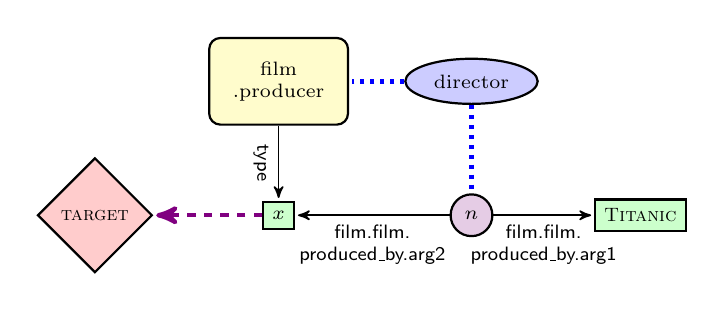
\begin{tikzpicture}[
  font=\sffamily,
  every matrix/.style={ampersand replacement=\&,column sep=0.7cm,row
sep=0.4cm,font=\scriptsize},
  entity/.style={draw,thick,rectangle,fill=green!20},
  word/.style={draw,thick,ellipse,fill=blue!20},
  mediator/.style={draw,thick,circle},
  mediatorR/.style={draw,thick,circle,fill=cyan!20},
  mediatorV/.style={draw,thick,circle,fill=violet!20},
  mediatorY/.style={draw,thick,circle,fill=yellow!20},
  entityType/.style={draw,thick,rounded corners,fill=yellow!20,inner sep=.3cm},
  mathType/.style={draw,thick,diamond,fill=red!20,font=\sc\scriptsize},
  mediatorToEntity/.style={->,>=stealth',shorten
>=1pt,semithick,black,sloped,above,font=\sffamily\scriptsize},
  typeToEntity/.style={->,>=stealth',shorten
>=1pt,semithick,black,sloped,above,font=\sffamily\scriptsize},
  wordToEntity/.style={-,>=stealth',shorten >=1pt,ultra
thick,dotted,blue,sloped,above,font=\sffamily\scriptsize},
  entityToMath/.style={->,>=stealth',shorten >=1pt,ultra
thick,dashed,violet,sloped,above,font=\sffamily\scriptsize},
  every node/.style={align=center}] 

  % Austin is the capital of Texas 
  
  % Position the nodes using a matrix layout
  \matrix{ 
  \& \node[entityType] (tCapital) {film\\.producer}; \& \node[word]
(wCapital) {director}; \\
    \node[mathType] (mTarget) {target}; \&  \node[entity] (eAustin) {$x$}; \& \node[mediatorV]
(mCapital) {$n$}; \& \node[entity]
(eTexas) {$\textsc{Titanic}$}; \\ 
  };
 
  % words to entities
  %\draw [wordToEntity] (wAustin) edge node {}  (eAustin);
  % \draw [wordToEntity] (wTexas) edge node {}  (eTexas);
  % words to types
  \draw [wordToEntity] (wCapital) edge node {}  (tCapital);
  
  % type to entity
  \draw [typeToEntity][below] (tCapital) edge node {type}  (eAustin);
  
  % event word to mediators
  \draw [wordToEntity] (wCapital) edge node {}  (mCapital);
  
  % mediator to entities
  \draw [mediatorToEntity][below] (mCapital) edge node {film.film.\\produced\_by.arg2}  (eAustin);
  \draw [mediatorToEntity][below] (mCapital) edge node {film.film.\\produced\_by.arg1}  (eTexas);
   
   \draw [entityToMath] (eAustin) edge node {}  (mTarget);
  
\end{tikzpicture} 
\scriptsize $\textsc{target}(x) \wedge \mbox{film.producer}(x) \wedge 
\mbox{film.film.produced\_by.arg2}(n, x) \wedge
\mbox{film.film.produced\_by.arg1}(n, \textsc{Titanic})$
\end{center}

% \end{landscape}

% \begin{tikzpicture}
% \node (One) at (-3,0) [shape=circle,draw] {$One$}; 
% \node (Two) at (3,0) [shape=circle,draw] {$Two$};
% \def\myshift#1{\raisebox{-2.5ex}}
% \draw [->,thick,postaction={decorate,decoration={text along path,text
%align=center,text={|\sffamily\myshift|Some more bent text}}}] (One) to [bend right=45]  (Two);
% \def\myshift#1{\raisebox{1ex}}
% \draw [->,thick,postaction={decorate,decoration={text along path,text
%align=center,text={|\sffamily\myshift|Some bent text}}}]      (One) to [bend left=45] (Two);
% \end{tikzpicture}


\end{document}
